%Apendice A
%
\chapter{Norma de cálculo en madera - NCh1198}
\label{ch:anexo_a}

La norma NCh 1198 - Cálculo de construcciones en madera - establece los métodos y procedimientos de diseño estructural que determinarán las condiciones mínimas que debe cumplir cada elemento de la estructura. Esta incluye las construcciones de madera aserrada, elaborada, laminada-encolada y postes de madera, como también las uniones a través de elementos mecánicos, tales como: clavos, tirafondos, pernos, barras de acero, tornillos y conectores para madera.

\section{Propiedades de la madera y factores de modificación}
\subsection{Contenido de humedad}
\label{sec:contenido_humedad}

El contenido de humedad de una madera debe ser considerado por su susceptibilidad a los cambios de forma, volumen y para la determinación de las tensiones admisibiles debido a que es un material higroscópico. Para esto, se debe tomar en cuenta su humedad durante la construcción ($H_c$), como también, la humedad a la que estará en servicio ($H_s)$ o humedad de equilibrio. La humedad de equilibrio depende de la ubicación que tengan los elementos. Si se encuentra en un recinto cerrado sin calefacción o intermitente $H_s= 12\%$. Si es un recinto cerrado continuamente calefaccionado, entonces $H_s=9\%$. Si es un recinto cubierto abierto, entonces la humedad de equilibrio será igual a la humedad medida del lugar donde se ubicará. Finalmente, si los elementos se encuentran a la interperie, se puede utilizar la tabla que se encuentra en el anexo D, de la norma NCh 1198, para las diferentes regiones geográficas de Chile.\\

Así la tabla \ref{tab:tabla3_1198} se utiliza de criterio para clasificar la madera como verde o seca, las cuales se designan con las letras E y ES, respectivamente. Además, son agrupadas con un número que clasifica las especies madereras que crecen en Chile, de acuerdo a la norma NCh 1989 - Agrupamiento de especies madereras según su resistencia - mostrada en el anexo A de la norma NCh 1198. Para el pino radiata se considera la clasificación de la norma NCh 1207 - Pino radiata, clasificación visual para uso estructural, especificaciones de los grados de calidad.

\begin{table}[h]
\centering
\resizebox{\textwidth}{!}{%
\begin{tabular}{@{}ccccc@{}}
\toprule
\multirow{2}{*}{Item} & \multicolumn{2}{c}{\begin{tabular}[c]{@{}c@{}}Condición de humedad \\ de la madera\end{tabular}} & \multicolumn{2}{c}{\begin{tabular}[c]{@{}c@{}}Condición considerada para la madera\\  en la determinación de su(s)\end{tabular}} \\ \cmidrule(l){2-5} 
                      & Durante la construcción                              & En servicio                                  & Tensiones admisibles                                           & Módulo de elasticidad                                           \\ \midrule
1                     & $H_c \geq 20\%$                                      & $H_s \geq 20\%$                              & Verde                                                          & Verde                                                           \\
2                     & $H_c \geq 20\%$                                      & $H_s \leq 12\%$                              & Seca (H=12\%)                                                  & Seca (H=12\%)                                                   \\
3                     & $H_c \leq 12\%$                                      & $H_s \leq 12\%$                              & Seca (H=12\%)                                                  & Seca (H=12\%)                                                   \\
4                     & $H_c \leq 12\%$                                      & $H_s \geq 12\%$                              & Verde                                                          & Seca (H=12\%)                                                   \\ \bottomrule
\end{tabular}%
}
\caption{Condiciones que se deben considerar en la determinación de tensiones admisibles y módulo de
elasticidad. \cite{nch1198}}
\label{tab:tabla3_1198}
\end{table}

\subsection{Densidad}
Debido a la característica higroscópica de la madera, su masa y volumen varían respecto al contenido de humedad. Por lo tanto, existen distintos tipos de densidad dependiendo de la información que sea necesaria o de los cálculos que se realicen. De acuerdo a la norma NCh 176/2, se definen los siguientes valores de densidad:
\begin{itemize}
	\item Densidad anhidra: Relaciona la masa y el volumen de la madera completamente seca (anhidra)
	\item Densidad normal: Aquella que relaciona la masa y el volumen de la madera con un contenido de humedad del 12\%.
	\item Densidad básica: Relaciona la masa anhidra de la madera y su volumen con humedad igual o superior al 30\%.
	\item Densidad nominal: Es la que relaciona la masa anhidra de la madera y su volumen con un contenido de humedad del 12\%.
	\item Densidad de referencia: Aquella que relaciona la masa y el volumen de la madera ambos con igual contenido de humedad.
\end{itemize}

\subsection{Tensiones admisibles y módulo de elasticidad}
La madera es un material no homogéneo constituido por fibras naturales que mantienen su dirección, las cuales inciden en que su comportamiento mecánico, su flexibilidad y la resistencia a los esfuerzos sea distinta respecto al eje en que se usa, siendo un material ortotrópico donde su resistencia es mayor en el eje paralelo a las fibras que el normal a las fibras.

Además, sus propiedades varían respecto a la especie del árbol, su edad, condiciones climáticas, humedad y la presencia de defectos, como nudos, rajaduras o agujeros. Para esto, la norma NCh 1970/1 y 1970/2 - Clasificación visual para uso estructural, especificaciones de los grados de calidad - junto a la norma NCh 1207, determinan el grado estructural desde el N$^\circ$1 al N$^\circ$4, a partir de una inspección visual de la madera procesada. Con esta clasificación, junto a la clasificación de madera seca o verde, determinan la clase estructural de la madera aserrada. Finalmente, con esta información es posible obtener la tensión admisible en flexión ($F_f$), compresión paralela a las fibras ($F_{cp}$), tracción paralela a las fibras ($F_{tp}$), cizalle ($F_{cz}$), compresión normal a las fibras ($F_{cn}$) y el módulo de elasticidad en flexión ($E_f$), de las tablas 4.a para todas las especias y 4.b para el pino radiata.

\subsection{Factores de modificación}
Existen otras variables externas a la madera que pueden afectar su correcto desempeño. Para esto, existen los factores de modificación que buscan corregir la tensión admisible para las distintas condiciones a las que puede estar sometido el elemento. Estas son:
\begin{itemize}
	\item Factor de modificación por contenido de humedad, $K_H$.
	\item Factor de modificación por duración de la carga, $K_D$.
	\item Factor de modificación por trabajo conjunto, $K_C$.
	\item Factor de modificación por temperatura.
	\item Factor de modificación por tratamiento químico
\end{itemize}

\section{Diseño de piezas}
Para el diseño de piezas es necesario calcular las tensiones de diseño, que se determinan como el producto de las tensiones admisibles por los factores de modificación que resulten pertinentes y que se definen para cada tipo de solicitación a la que está sometida cada pieza de la estructura. Por lo tanto, las tensiones de trabajo no pueden ser superiores a las de diseño, debiendo establecerse, un factor de seguridad para los cálculos. A continuación se expondrán las solicitaciones utilizadas para el diseño de la mesa.

\subsection{Flexión}
La tensión de trabajo de flexión de la fibra extrema de una viga simple de madera se debe determinar de acuerdo con la expresión:
\begin{equation} \label{eq:f_f}
	f_f=\frac{M_{max}}{W_n} \qquad \text{(MPa)}
\end{equation}

Donde $M_{max}$ es el momento máximo de flexión en $\text{N}\cdot\text{mm}$ y $W_n$ el módulo de flexión de la sección transversal neta respecto al eje neutro en mm.

Para el diseño de elementos en flexión, se debe calcular la tensión de diseño en flexión en la zona flexo-traccionada ($F_{ft,dis}$) y flexo-comprimida ($F_{fv,dis}$). Que se definen según las ecuaciones \ref{eq:ft_dis} y \ref{eq:fv_dis}.
\begin{subequations}
\begin{align}
	F_{ft,dis}&=F_f \cdot K_H \cdot K_D \cdot K_C \cdot K_{hf} &\text{(MPa)} \label{eq:ft_dis}\\	
	F_{fv,dis}&=F_f \cdot K_H \cdot K_D \cdot K_C \cdot K_V &\text{(MPa)}	 \label{eq:fv_dis}
\end{align}
\end{subequations}

Donde:
\begin{itemize}
	\item[] $K_{hf}$: Factor de modificación por altura.
	\item[] $K_V$: Factor de modificación por volcamiento.
\end{itemize}

\subsubsection{Factor de modificación por altura, $K_{hf}.$}
Para todas las especies forestales, con excepción del pino radiata, en piezas traccionadas o vigas rectangulares de ancho o altura superior de 50 mm, este factor se evualúa de acuerdo con la expresíon \ref{eq:khf}. Para pieza de Pino radiata de altura superior a 90 mm, se considera la expresión \ref{eq:khf}.

\begin{subequations}
\begin{align}
	K_{hf}&=\left(\frac{50}{h}\right)^{\frac{1}{9}} \label{eq:khf}\\
	K_{hf,radiata}&=\left(\frac{90}{h}\right)^{\frac{1}{5}} \label{eq:khfr}
\end{align}
\end{subequations}

Donde $h$ es el ancho de la viga traccionada o altura de la viga, en mm.
\subsubsection{Factor de modificación por volcamiento, $K_V.$} Aquellos elementos estructurales que estén sometidos a flexión deben estar apoyados laterlamente en sus extremos para impedir desplazamientos laterales y rotaciones en el eje axial, donde se denomina luz a la distancia entre puntos de apoyo de un elemento de estructura. Para esto existen tres posible casos dependiendo de la configuración, donde $h$ es la altura de la viga y $b$ su ancho.
\begin{enumerate}
	\item Cuando los elementos en flexión cumplen con las especificaciones de la \textbf{Tabla 11}, de la sección \textbf{8.2.2.4} de la norma, $K_V= 1$.
	\item Si los elementos no poseen apoyos laterales a lo largo de su luz, $K_V = 1$, si la razón $(h/b) < 2$.
	\item Si en el punto anterior $(h/b) > 2$, $H_V$ se calcula en función de la esbeltez de volcamiento $\lambda_V$, de acuerdo a la sección \textbf{8.2.1.8}, la \textbf{Tabla 10} y \textbf{Tabla 12} de la norma.
\end{enumerate}

En aquellos casos en los que la esbeltez de volcamiento ($\lambda_V$) sea mayor a la esbeltez del límite elástico ($\lambda_{vo}$), el factor de modificación se calcula como:
\begin{equation}\label{eq:k_v}
	K_v = \frac{0,4\cdot E_{f,dis}}{\lambda_{v}^2 \cdot F_{f,dis}'}
\end{equation}

\subsection{Cizalle en vigas simples}
La tensión de trabajo máximo de cizalle longitudinal en elementos flexionados de madera, se calcula mediante la siguiente expresión:

\begin{equation} \label{eq:f_cz}
f_{cz} = \frac{1,5 \cdot Q}{b \cdot h} \qquad \text{(MPa)}
\end{equation}
\\
Donde $Q$ es el esfuerzo cortante máximo y $b$ y $h$ la base y altura en mm, respectivamente. La tensión de diseño de cizalle longitudinal se determina de la expresión \ref{eq:cz_dis} . El cizalle transversal no es necesario calcular o verificar debido a que nunca va a fallar por este esfuerzo, según la sección \textbf{8.2.3.1} de la norma.

\begin{equation}\label{eq:cz_dis}
	F_{cz.dis} = F_{cz} \cdot K_H \cdot K_D \cdot K_C \cdot K_r \qquad \text{(MPa)}
\end{equation}

Donde $K_r$ es el factor de modificación por rebaje (inferior o superior), calculado según la sección \textbf{8.2.3.5}. Debido a que no es una condición que se encuentra en este trabajo, no se profundizará en este factor.\\


\subsection{Compresión paralela a la fibra}
\label{sec:cp}
La tensión de trabajo de una columna simple sometida a compresión paralela a su fibra, se calcula:
\begin{equation}\label{eq:f_cp}
	f_{cp}= \frac{N}{A} \cdot 10^{-3} \qquad \text{(MPa)}
\end{equation}

Donde N es la carga axial aplicada en kN, y A el área de la sección transversal en mm$^2$. 

El cálculo de la tensión de diseño en compresión paralela ($F_{cp,dis}$) dependerá de la inestabilidad lateral ($\lambda$), la cual, dependiendo de su valor, será necesario calcular un factor de modificación por esbeltez, como también pondrá restricciones al diseño. Así, se puede obtener $F_{cp,dis}$ a partir de las ecuaciones \ref{eq:cp_dis} y \ref{eq:cp_dislambda}. 

La esbeltez se define como $\lambda = l_p/i$, donde $l_p$ es la longitud efectiva de pandeo, e $i$ corresponde al radio de giro. Para el cálculo de la longitud efectiva de pandeo, se pueden utilizar los valores de la \textbf{Tabla 18} o las recomendaciones establecidas en el anexo K, según la norma.
\begin{subequations}
\begin{align}
	F_{cp,dis} &= F_{cp} \cdot K_H \cdot K_D \cdot K_C \label{eq:cp_dis}\\
	F_{cp,\lambda,dis} &= F_{cp,dis} \cdot K_{\lambda} \label{eq:cp_dislambda}
\end{align}
\end{subequations}
Donde $K_{\lambda}$ es el factor de modificación por esbeltez. Si $\lambda < 5$, la tensión de diseño se calculará según \ref{eq:cp_dis}. Por otro lado, si $\lambda \geq 5$, entonces determina mediante la ecuación \ref{eq:cp_dislambda} debido a que el elemento presenta inestabilidad lateral.

El factor $K_{\lambda}$ se evalúa según la expresión:
\begin{equation}\label{eq:k_lambda}
	K_{\lambda} = A - \sqrt{A^2 - B}
\end{equation}
con:
\begin{gather}
	A = \frac{B\cdot c\cdot (1 + \frac{\lambda}{200}) + 1}{2\,c}
\end{gather}
\vspace{-8mm}
\begin{gather}
	B = \frac{4\, E_{dis}}{c\cdot \lambda^2\cdot F_{cp,dis}}
\end{gather}
en que:
\begin{itemize}
	\item $c\:$: Corresponde al coeficiente de proporcionalidad y cuyos valores se obtienen de la tabla 19 de la norma a partir del grado estructural de la madera.
	\item $E_{dis}\,$: Módulo elástico de diseño, calculado como el módulo elástico en flexión $E_f$ por los factores de modificación que resulten pertinentes.  
	\item $F_{cp,dis}\,$: Tensión de diseño en compresíon paralela calculada según \ref{eq:cp_dis}, excluyendo el factor de modificación por trabajo conjunto, $K_C$, en MPa.
\end{itemize}

\subsection{Compresión normal a la fibra}
La tensión de trabajo por aplastamiento en superficies de apoyo, solicitadas ortogonalmente a la fibra, se determina según la siguiente expresión:
\begin{equation}
	f_{cn}= \frac{R}{A_n} \qquad \text{(MPa)}
\end{equation}

Donde $R$ es la carga aplicada y $A_n$ la sección neta aplastada.

La tensión de diseño en compresión normal, se calcula a partir de la siguiente expresión:
\begin{equation}
	F_{cn,dis} = F_{cn} \cdot K_H \cdot K_C \cdot K_{cn}
\end{equation}
Donde $K_{cn}$ es el factor de modificación por aplastamiento, que se calcula a partir de la sección \textbf{8.5.3} de la norma.


\section{Nomenclatura y tipos de madera}
Más allá de la especie, en el mercado es posible encontrar madera con distintas terminaciónes y dimensiones. Las principales diferencias se definen respecto al grado de manipulación del material y su uso final. Los tipos de madera relevantes a este trabajo son los siguientes:
\begin{itemize}
	\item Madera dimensionada: Tal como dice su nombre, es una madera cortada sin cepillar, conservando sus dimensiones en bruto.
	\item Madera cepillada: Es el siguiente paso a la madera dimensionada. Recibe su nombre por el uso de la herramienta cepillo, la cual desbasta la superficie de la madera para suavizarla. Este formato mantiene sus dimensiones nominales en bruto, sin embargo, pierde sección respecto a la madera dimensionada.
	\item Madera laminada: También conocida como laminada-encolada, es la unión de tablas similares, de canto o de tope, manteniendo la misma dirección de las fibras, utulizando adhesivos sobre sus caras.
\end{itemize}

Por otro lado, existen distintas configuraciones dependiendo de la escuadría y la forma de la sección \cite{sistemasconstructivos}:
\begin{itemize}
	\item Listón: Elemento de escuadría 1x2'', 2x2'', 2x3'' y 2x4''.
	\item Tabla: Elemento donde prevalece el alto por sobre el espesor, comúnmente de escuadrías 1x4'', 1x5'' o 1x6''.
	\item Tablón: Elemento más grueso que una tabla, de escuadría 2x6'', 2x8'' o 2x10''.
	\item Cuartón: Elemento de sección cuadrada. Su nombre se debe a la sección 4x4'', pero puede ser de 5x5'' o 6x6''.
	\item Base: Elemento de escuadría de 10x10'' o superior. 
\end{itemize}

Todas las dimensiones, independiente del formato o el tipo, son respecto a la madera en bruto. Por lo tanto, a pesar que las dimensiones reales de una madera cepillada o dimensionada son menores, se sigue denominando según su escuadría original. Así, las tablas \ref{tab:anchodim} y \ref{tab:espdim} muestran los valores reales para cada dimensión nominal.

\begin{table}[H]
\centering
\begin{tabular}{@{}cccc@{}}
\toprule
\multirow{2}{*}{Espesor Nominal {[}in{]}} & \multicolumn{2}{c}{Dimensionado {[}mm{]}} & Cepillado {[}mm{]} \\ \cmidrule(l){2-4} 
                                  & Verde                & Seco               & Seco               \\ \midrule
1                                 & 23                   & 22                 & 19                 \\
2                                 & 48                   & 45                 & 41                 \\ \midrule
Tolerancia {[}mm{]}               & 0/+2                 & 0/+3               & 0/+2               \\ \bottomrule
\end{tabular}
\caption{Espesor nominal y real de la madera según el tratamiento recibido.}
\label{tab:espdim}
\end{table}

\begin{table}[H]
\centering
\begin{tabular}{@{}cccc@{}}
\toprule
\multirow{2}{*}{Ancho Nominal {[}in{]}} & \multicolumn{2}{c}{Dimensionado {[}mm{]}} & Cepillado {[}mm{]} \\ \cmidrule(l){2-4} 
                                        & Verde                & Seco               & Seco               \\ \midrule
2                                       & 48                   & 45                 & 41                 \\
3                                       & 73                   & 69                 & 65                 \\
4                                       & 99                   & 94                 & 90                 \\
5                                       & 127                  & 120                & 115                \\
6                                       & 150                  & 142                & 138                \\
8                                       & 200                  & 190                & 185                \\
10                                      & 248                  & 235                & 230                \\ \midrule
Tolerancia {[}mm{]}                     & 0/+2                 & 0/+3               & 0/+2               \\ \bottomrule
\end{tabular}
\caption{Ancho nominal y real de la madera según el tratamiento recibido.}
\label{tab:anchodim}
\end{table}

\section{Uniones en la madera estrutural}
Existen diversas formas de unir dos o más elementos de madera. Uno de ellos es el ensamble entre las piezas, en cual, modificando la geometría de ambos elementos, se busca unirlas sin añadir objetos externos. Sin embargo, actualmente se opta por el uso de elementos externos para unir elementos de tipo estructural. Así, la norma NCh 1198 dispone de un capítulo para el correcto uso de estos elementos mecánicos.
\subsection{Generalidades}
Antes de comenzar a hablar de las expresiones que determinan el comportamiento de las unionse mecácnicas, se deben realizar definiciones previas. 
\begin{enumerate}
		\item Elementos mecánicos de unión: Son aquellos que, al quedar solicitados por fuerza de cizalle, admiten corrimientos relativos entre ls piezas conectadas. Dependiendo de su disposición pueden quedar solicitados en su dirección axial también.
		\item Borde cargado: Borde de la pieza de madera que se encuentra afectado por la acción de la fuerza que transmite el elemento de unión o por alguna de las fuerzas de las componentes de esta.
		\item Borde descargado: Borde que no está sometido a las fuerzas señaladas en el punto anterior.
		\item Espaciamientos: Es la distancia entre centros de elementos de unión adyacentes o entre centros de elementos de unión vecinos a un borde y éste, los que se clasifican de la siguiente manera:
		\begin{enumerate}
			\item Espaciamiento mínimo entre elementos de unión medido en dirección paralela a la fibra de la pieza: $s_p$.
			\item Espaciamiento mínimo entre elementos de unión medido en dirección normal a la fibra de la pieza: $s_n$.
			\item Espaciamiento mínimo entre un elemento de unión y un borde cargado medido en dirección paralela a la fibra de la pieza: $s_{bcp}$.
			\item Espaciamiento mínimo entre un elemento de unión y un borde cargado medido en dirección normal a la fibra de una pieza: $s_{bcn}$.
			\item Espaciamiento mínimo entre un elemento de unión y un borde descargado medido en dirección paralela a la fibra de la pieza: $s_{bdp}$.
			\item Espaciamiento mínimo entre un elemento de unión y un borde descargado medido en dirección normal a la fibra de la pieza: $s_{bdn}$.
		\end{enumerate}
		Y se muestran en la figura \ref{fig:nch_17}.
		\item Duración de la carga: Las cargas admisibles definidas en este capítulo son aplicables para cargas de una duración de 10 años. Para valores distintos, se se debe seguir las indicaciones de la sección \textbf{7.1.2}.
		\item Extracción directa: Se refiere a cuando una unión está siendo solicitada axialmente respecto al eje del elemento de unión. 
		\item Extracción lateral: Se refiere a cuando una unión está siendo solicitada perpendicularmente al eje del elemento de unión, sometiendolo a esfuerzos de cizalle en su sección transversal, siendo el tipo de solicitación más común.
		\item Condición de la madera: En relación a los medios de unión, se define respecto al contenido de humedad (H) en la madera, así se establecen tres casos:
		\begin{enumerate}
			\item Seca: Si su contenido de humedad es menor a 20\% (H < 20\%).
			\item Semiseca: Si su contenito de humedad está comprendido entre 20\% y el punto de saturación de la fibra (P.S.F.), (20\% $\geq$  PSF).
			\item Verde: Si su contenido de humedad es igual o superior a PSF. (H $\leq$ PSF)
		\end{enumerate}
		\item Punto de saturación de la fibra (PSF): Corresponde al valor del contenido de humedad en el cual una madera ha perdido teóricamente toda su agua libre y sus paredes celulares están saturadas de agua higroscópica, representando el punto donde la madera se comprime o hincha, en procesos de secado o adsorción respectivamente. Su valor depende de distintos factores, como el tipo de secado o el tipo de madera, sin embargo, la norma asume un valor H = 28\% como PSF.
\end{enumerate}

Las cargas admisibles especificadas en el capítulo 10 de la norma son para uniones colocadas en madera seca y que se mantendrá seca después de su construcción. Para madera semiseca o verde durante su construcción y madera seca que durante su servicio aumenta su contenido de humedad por sobre el 19\%, se le deberá aplicar el factor de modificación $K_{UH}$ señalado en las tablas 28 y 29, de la sección \textbf{10.1.7} de la norma.

\begin{figure}[p]
\centering
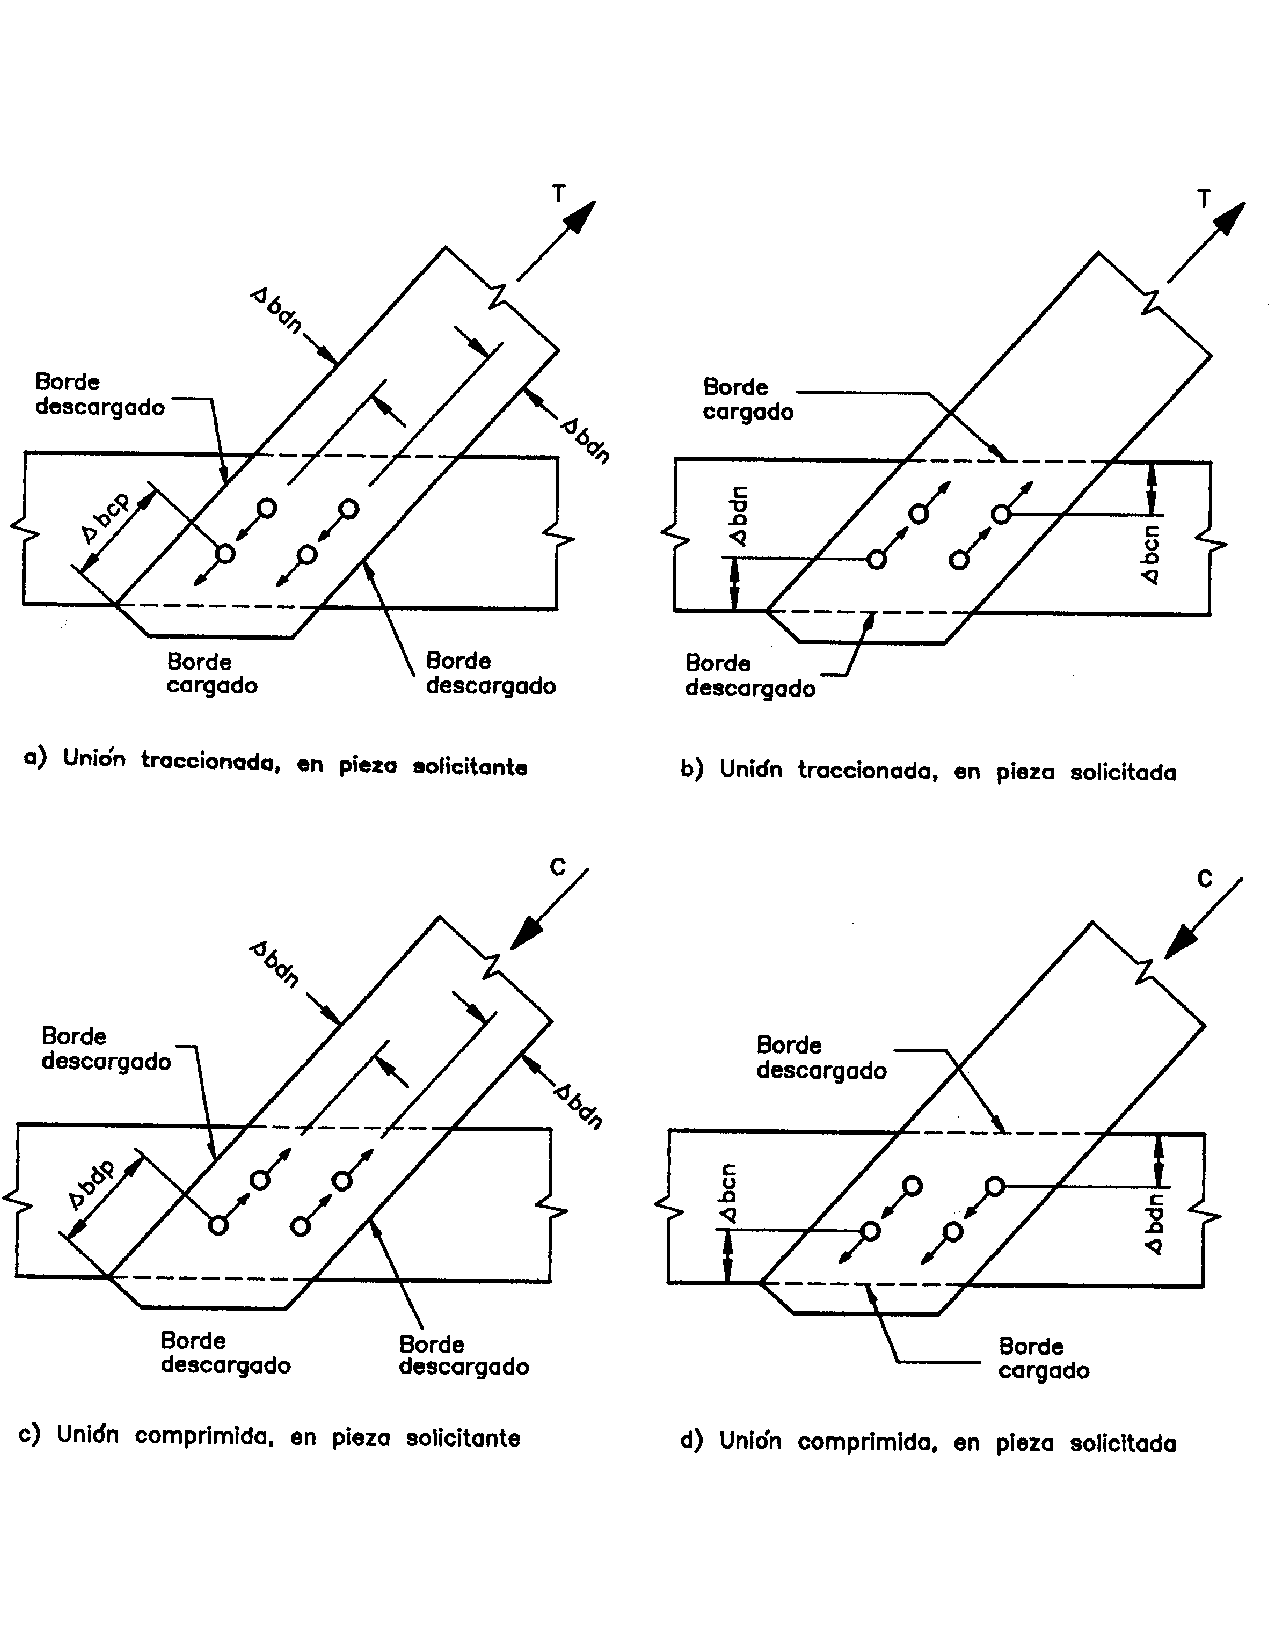
\includegraphics[width=1\linewidth, angle=1,origin=c]{Imagenes/figura_17.pdf}
\caption{Designaciones de espaciamientos y bordes. \cite{nch1198}}
\label{fig:nch_17}
\end{figure}

\subsection{Verificaciones tensionales}
\subsubsection{Sección transversal neta}
La capacidad soportante de carga de las piezas debe verificarse en la menor sección transversal neta que condiciona la ejecución de las uniones, deduciendo de la sección transversal bruta las áreas de perforaciones o de cualquier otra remoción de madera.\\
Así, el área neta requerida en piezas traccionadas y comprimidas, se determina dividiendo la carga total que se traspasa a través de la sección transversal neta crítica, por los correspondientes valores de diseño $F_{tp,dis} $ o $F_{cp,dis}$. Para las solicitaciones donde existen elementos de unión alineados de forma alternada, estos se deben considerar dispuestos en una misma sección transversal, a excepción que el espaciamiento entre estos sea mayor o igual a:
\begin{itemize}
	\item 8 diámetros para pernos, barras de acero y tirafondos.
	\item 2 diámetros en caso de conectores.
\end{itemize}

\subsubsection{Tensiones de cizalle}
En uniones de pernos, barras de acero, tirafondos o conectores, solicitadas por fuerzas de corte, se debe verificar que las tensiones de cizalle de trabajo $f_{cz}$ no excedan los siguientes valores indicados:
\begin{itemize}
	\item En uniones separadas del extemo de la pieza, por una distancia $s_{bp}$ mayor o igual que 5 veces la altura de la misma: 
	\begin{equation}
		f_{cz} = \frac{3\cdot Q}{2\cdot b\cdot h_e} \leq 1,5\cdot F_{cz,dis}  
	\end{equation}
	\item En uniones separadas del extremo de la pieza, por una distancia $s_{bp}$ menor que 5 veces la altura de la misma:
	\begin{equation}
		f_{cz} = \frac{3Q}{2 b h_e} \frac{h}{h_e} \leq F_{cz,dis}
	\end{equation}
	\item Se debe verificar que la sección transversal bruta cumple con la relación:
	\begin{equation}
		f_{cz} = \frac{3\cdot Q}{2\cdot b\cdot h} \leq F_{cz,dis}
	\end{equation}		
\end{itemize}

Los valores $h$ y $h_e$ se muestran en la figura \ref{fig:nch_19}. El valor $h_e$ será distinto para conectores o para pernos, barras de acero y tirafondos. Para conectores $h_e$ corresponde a la altura de la pieza menos la distancia desde el borde descargado hasta el borde del conector más cercano, mientras que en el caso del resto de las uniones, se evalúa deduciendo de la altura, la distancia entre el borde descargado y el centro de la unión más próxima.

\begin{figure}[H]
\centering
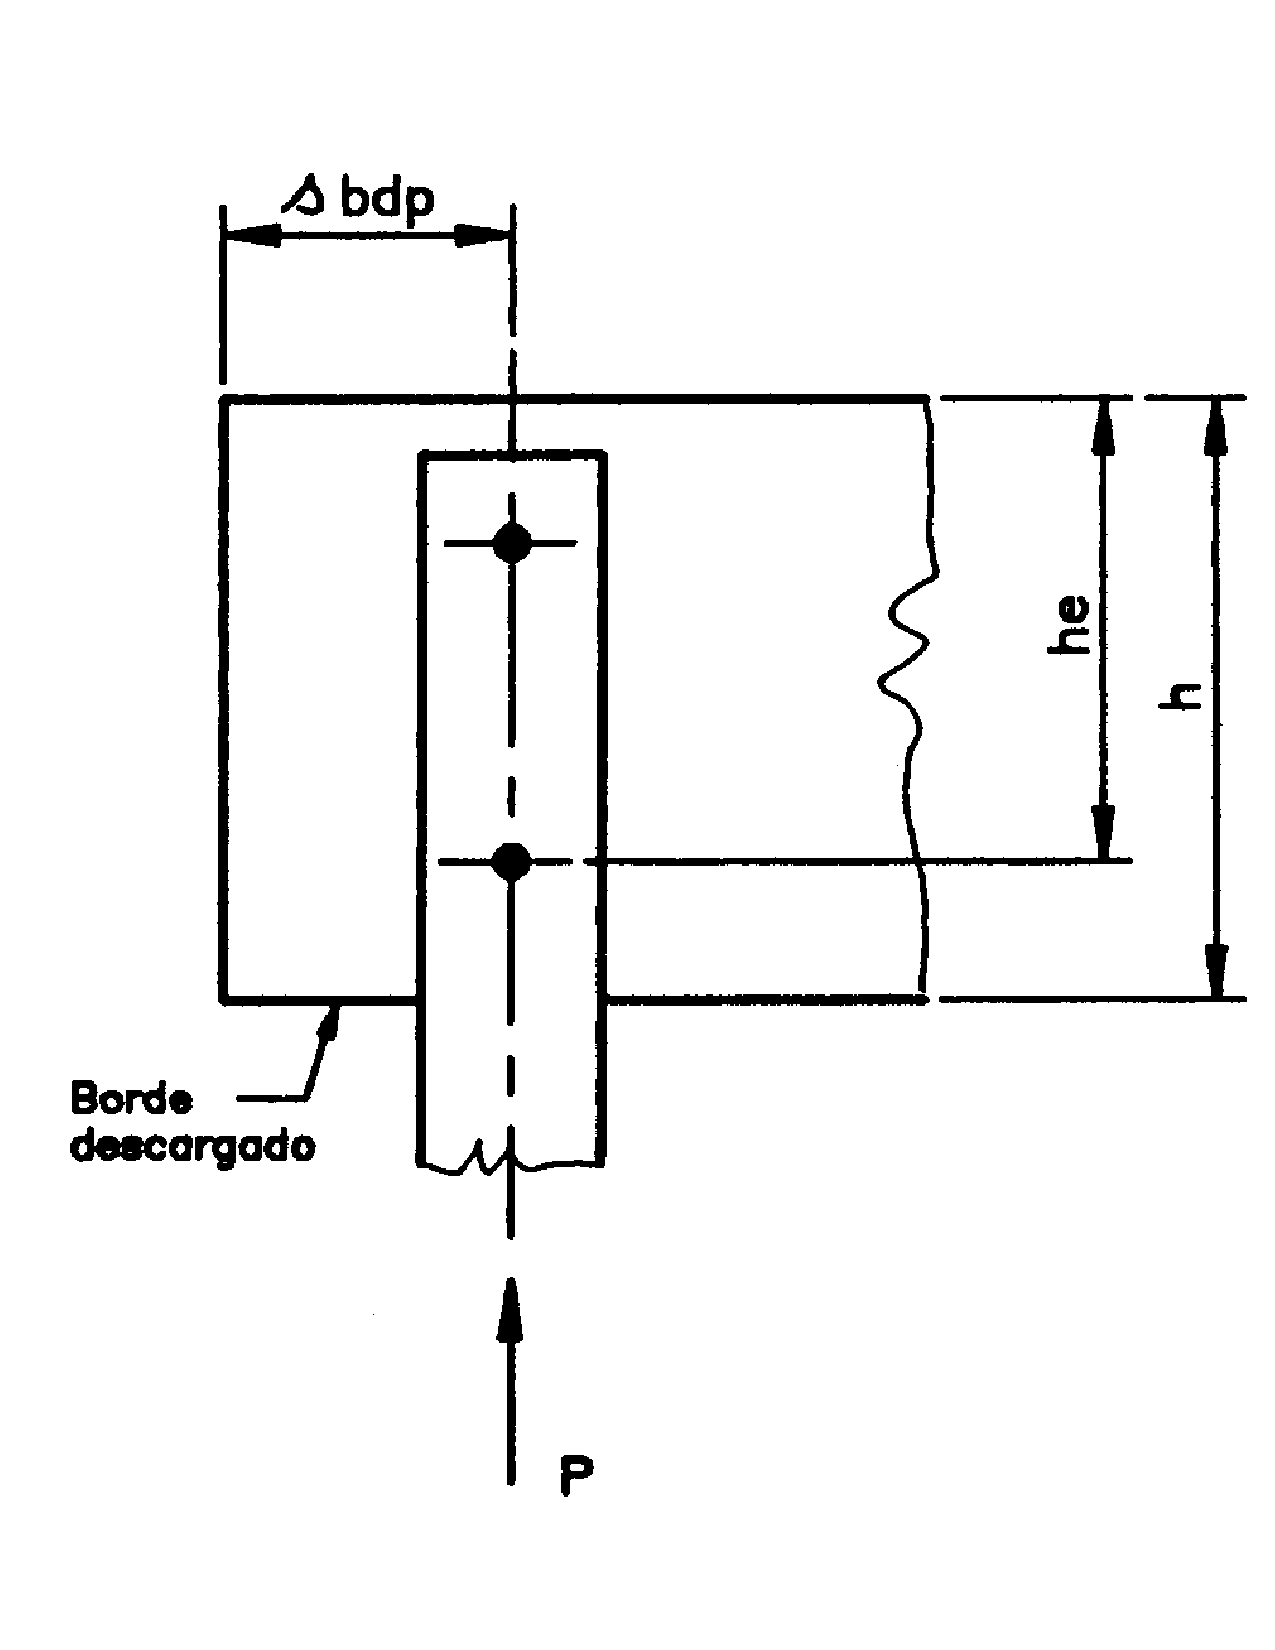
\includegraphics[width=0.45\linewidth]{Imagenes/figura_19.pdf}
\caption{Valor de $h_e$, para los distintos elementos de unión. \cite{nch1198}}
\label{fig:nch_19}
\end{figure}


\subsection{Número de elementos de unión}
Las cargas admisibles que se indican en esta norma, rigen para un elemento de unión individual, según las solicitaciones correspondientes. Una hilera de elementos de unión consiste en dos o más elementos del mismo tipo y tamaño alineados. En madera, es usual el uso de más de un elemento para unir dos o más maderas, debido a las restricciones existentes en su tamaño y distanciamiento.

\subsubsection{Carga admisible y factor de modificación por longitud de hilera}
La capacidad de carga admisible de una hilera es la suma de las capacidades de cada elemento que constituye la unión, sin embargo, no debe sobrepasar el valor $P_h$, determinado por la ecuación \ref{eq:adm_hilera}.

\begin{equation}\label{eq:adm_hilera}
	P_h = K_u \cdot \sum P_i
\end{equation}
Donde $\sum P_i$ es la suma de los valores admisibles de los elementos de unión individuales existentes en la hilera y $K_u$ es el factor de modificación por longitud de hilera, señalado en la sección \textbf{10.3.2.2} y las tablas 30 y 31 de la norma.

\subsection{Uniones con perno}
\label{sec:union_perno}
Las especificaciones para pernos son aplicables para cualquier elemento cilíndrico de acero que atreviese perpendicularmente los planos de cizalle de la unión y que quedan solicitados preponderantemente en flexión induciendo sobre la madera tensiones de aplastamiento.

Para su correcta instalación es necesario que los agujeros y las arandelas cumplan con ciertas dimensiones. El diámetro del agujero se debe mayorar respecto al del perno en función del tamaño del perno y las condiciones de humedad de servicio, siguiendo la tabla 33 de la sección \textbf{10.5.1.2} de la norma. Para las arandelas o golillas, se debe seleccionar primero si se utilizará una de forma circular o cuadrada, dando preferencia a esta última por ofrecer mayor resistencia al incrustramiento en la madera. Luego , sus respectivas dimensiones están en función del diámetro del perno, siguiendo la tabla 34 de la norma.

Respecto a las características del perno, su diámetro nominal debe estar entre los 10 y 30 mm. Además, se exige una disposición mínima de dos pernos, exceptuando los casos donde un único perno no queda solicitado en un porcentaje superior al 50\% de su capacidad de diseño.

\subsubsection{Cargas admisibles para un perno}
Las cargas admisibles para este tipo de unión solo son aplicables cuando la dirección de la solicitación es perpendicular a su eje para duración normal y de madera seca que permanecerá seca en servicio. Para casos distintos es necesario aplicar los factores de modificación correspondientes. Por otro lado, en esta norma existen condiciones distintas para cizalle simple, doble o múltiple, sin embargo, cizalle simple y múltiple se calculan realizando modificaciones al cizalle doble, por lo tanto, sólo se efectuara una explicación de este caso.

La capacidad de carga admisible ($P_{ad}$) se calcula estableciendo que la unión está establecida por la unión de tres piezas de la misma especia, con las piezas laterales paralelas entre sí y cada una de ellas de espesor igual a la mitad del espesor de la pieza central, e, como se muestra en la figura \ref{fig:nch_23}. Así, es posible obtenerla a través de la tensión admisible de aplastamiento nominal ,$F_{ap}$ (\ref{eq:f_ap}) , la esbeltez de la unión $\lambda_u$ y el diámetro del perno ($D$), de acuerdo a la siguiente expresión:
\begin{equation} \label{eq:padm_ad}
	P_{ad} = F_{ap} \cdot \lambda_u \cdot D^2 \leq Z \cdot D^2
\end{equation}

Y la tensión admisible de aplastamiento nominal se define como:
\begin{equation}\label{eq:f_ap}
	F_{ap} = \frac{0,00065\cdot \rho_{12,k}\cdot (100 - D)}{\eta (2,75\cdot \sin^2(\theta) + \cos^2(\theta)} \qquad \text{(MPa)}
\end{equation}


Donde:
\begin{align*}
&\rho_{12,k} &: \qquad &\text{Es la densidad normal característica de la especie forestal, en kg/m}^3 \text{, según}\\
& & & \text{tabla E2 del anexo E de la norma. D es el diámetro del perno, en mm.}\\
&D &: \qquad &\text{Diámetro del perno, en mm}\\
&\eta &: \qquad &\text{Es el factor de reducción de la zona elástica, según tabla 35 de la norma.}\\
&\theta &: \qquad &\text{Es la desangulación fuerza-fibra.}\\
&\lambda_u = \frac{e}{D} &: \qquad &\text{Esbeltez del perno en la pieza central}\\
&Z &= \qquad &1,15\cdot \sqrt{\frac{F_{ap} \cdot F_y}{\eta}} \qquad \text{(MPa)}\\
&F_y &: \qquad &\text{Tensión de fluencia del acero, usando 240 MPa como referencia} 
\end{align*}

\begin{figure}[H]
\centering
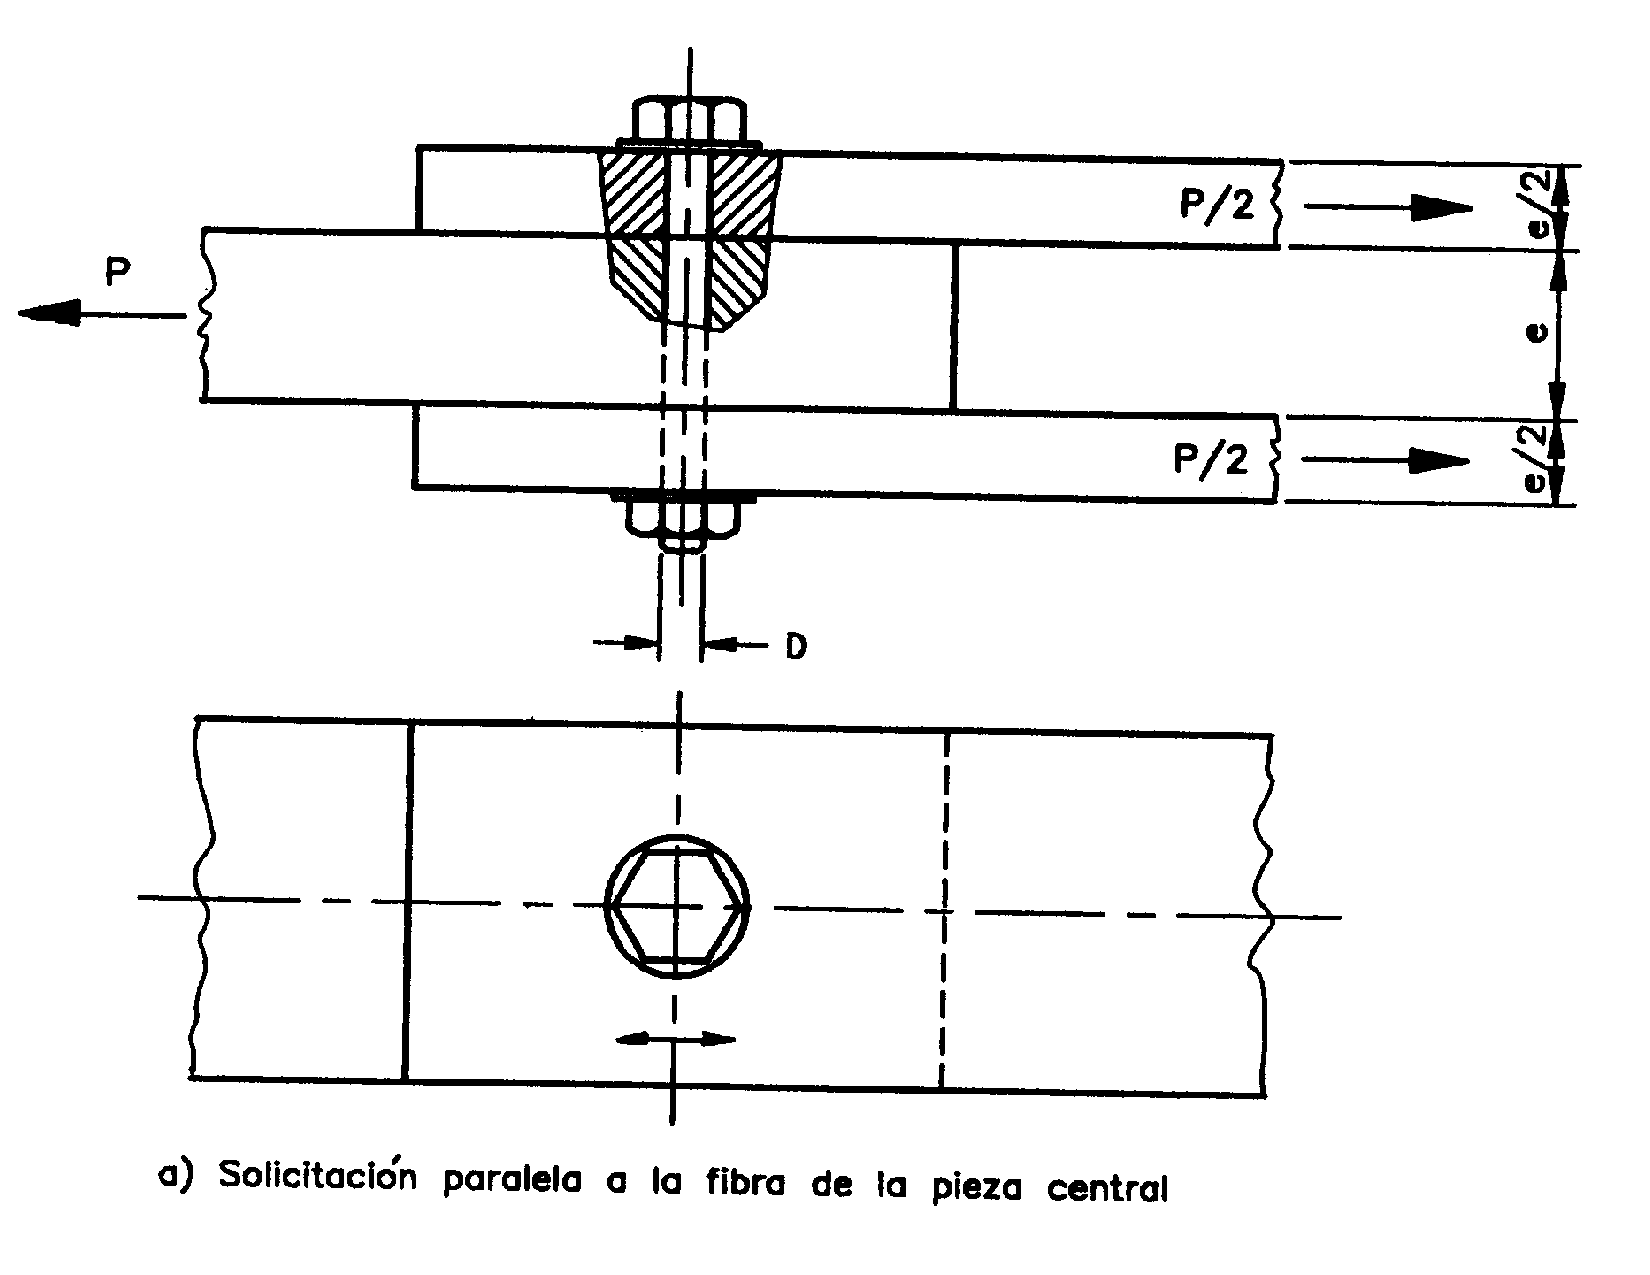
\includegraphics[width=0.5\linewidth, angle=1,origin=c]{Imagenes/figura_23A.pdf}%
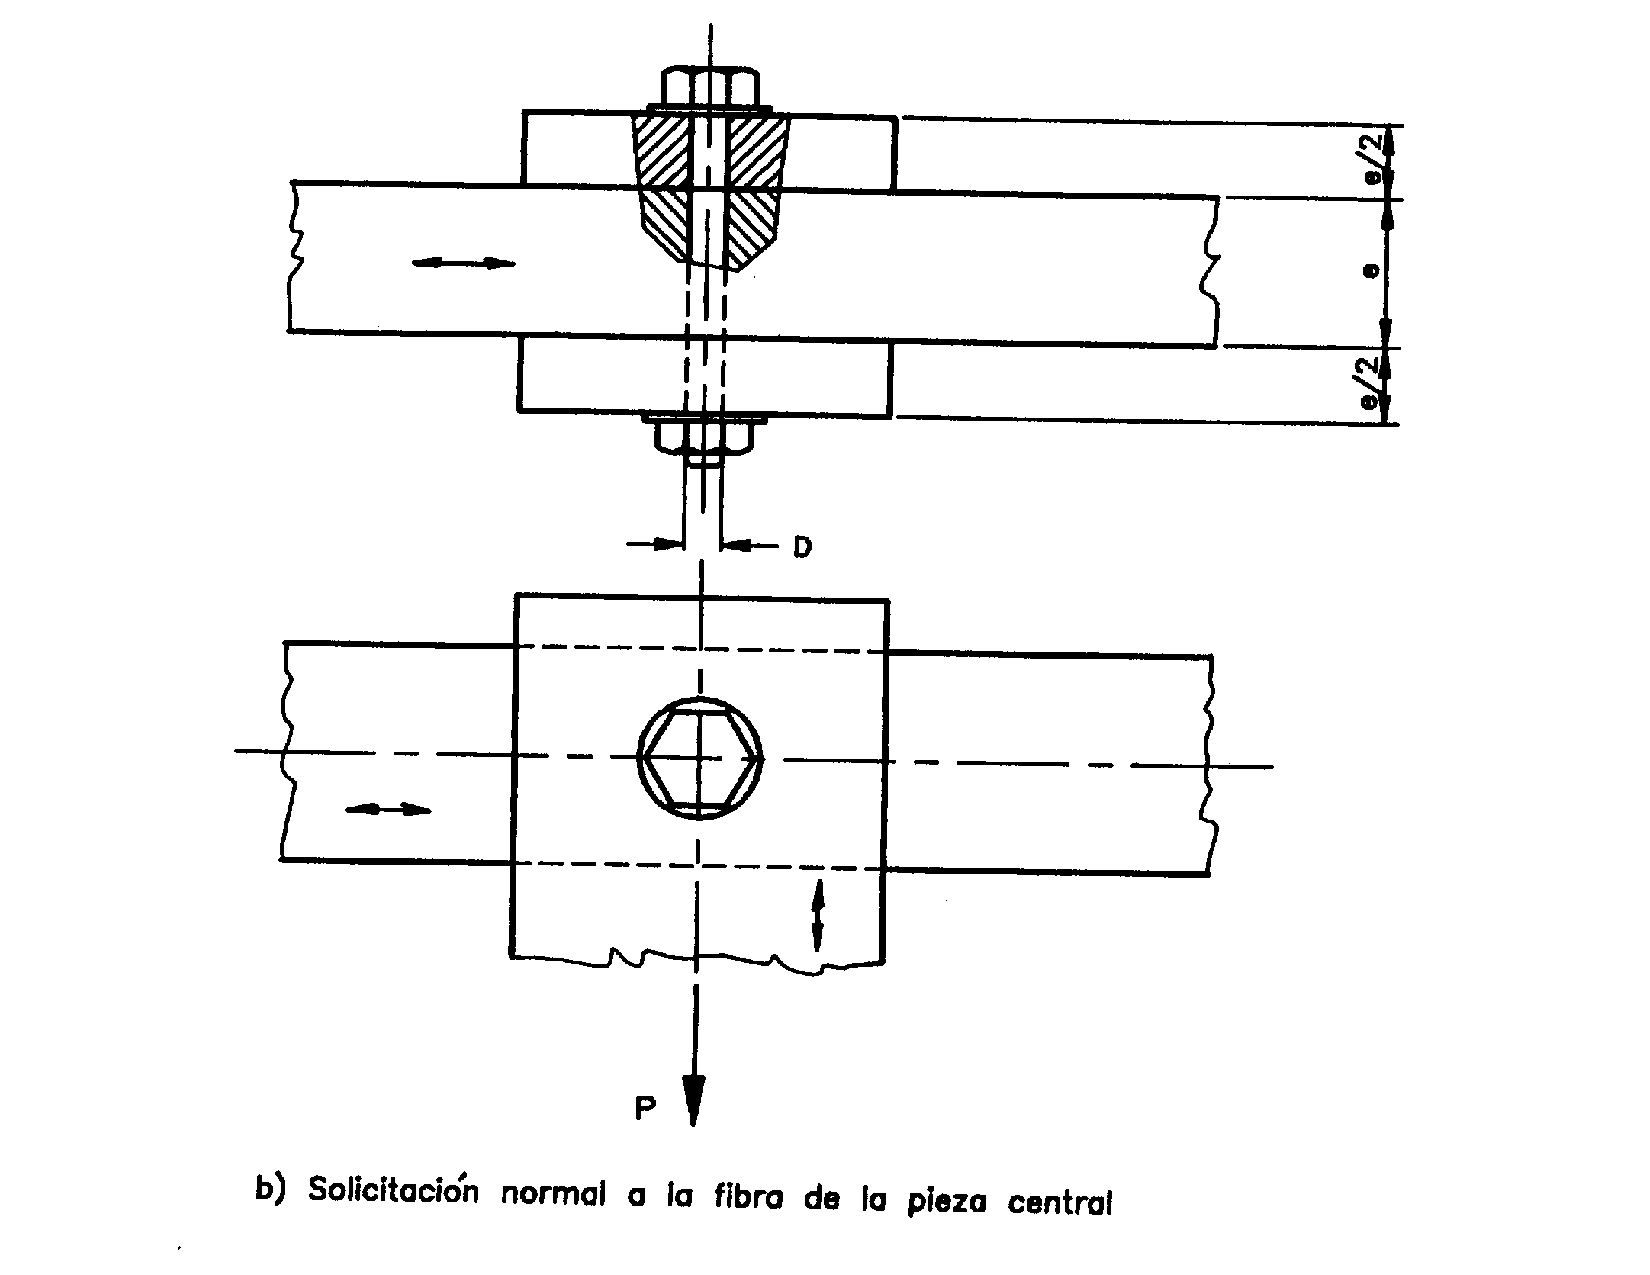
\includegraphics[width=0.5\linewidth, angle=1,origin=c]{Imagenes/figura_23B.pdf}
\caption{Uniones en cizalle doble. \cite{nch1198}}
\label{fig:nch_23}
\end{figure}


Para casos distintos al establecido anteriormente, se deben realizar arreglos en la forma de cálcular $P_{ad}$. En caso que las piezas laterales tengan un espesor menor que la mitad del espesor de la pieza central $e$, la carga admisibles es igual a la de una unión de cizalle doble con una pieza central de espesor ficticio, $e*$, equivalente al doble del espesor de la pieza lateral más delgada. Si las piezas laterales están constituidas de una especie maderera distinta a la pieza central, se debe considerar la menor entre:
\begin{itemize*}
	\item El valor determinado para una unión equivalente con todas sus piezas de la especie usada en las piezas laterales.
	\item El valor determinado para una unión equivalente con todas sus piezas constituidas con la especie de la pieza central.
\end{itemize*}

Cuando se usen planchas de acero como piezas laterales, las cargas admisibles para solicitaciones orientadas según la dirección de la fibra, se pueden mayorar en un 25\%, sin embargo estas mayoraciones no se permiten para las cargas admisibles calculadas con solicitaciones normales a la fibra.

El valor obtenido de $P_{ad}$ según la ecuación \ref{eq:padm_ad}, considera el eventual aflojamiento de tuercas inherentes a la contracción de la madera.

Finalmente, para cizalle simple existen dos casos a considerar. Cuando la unión está constituida por dos piezas de espesores diferentes, la carga admisible se determina como el menor valor entre:
\begin{itemize*}
	\item La mitad de la carga admisible de una unión de cizalle doble con una pieza central de espesor igual al de la pieza más gruesa.
	\item La mitad de la carga admisible de una unión de cizalle doble con una pieza central de espesor igual al doble del espesor de la pieza más delgada.
\end{itemize*}
El segundo caso, cuando las piezas son de igual espesor, la carga admisible equivale a la mitad de la correspondiente a la de una unión de cizalle doble con una pieza central de espsor igual al de cada pieza.

\subsubsection{Espaciamientos mínimos para pernos}
\label{sec:espaciamiento_pernos}
Los espaciamientos mínimos que se deben respetar en las uniones con pernos se esquematizan en la figura \ref{fig:nch_26}. El espaciamiento mínimo entre los pernos y los bordes cargados o descargados se establecen en función del diámetro del mismo, determinados por la tabla 36 de la sección \textbf{10.5.4} de la norma. El espaciamiento mínimo ente los pernos mismos, se establecen en la tabla 37 de la misma sección. 

\begin{figure}[p]
\centering
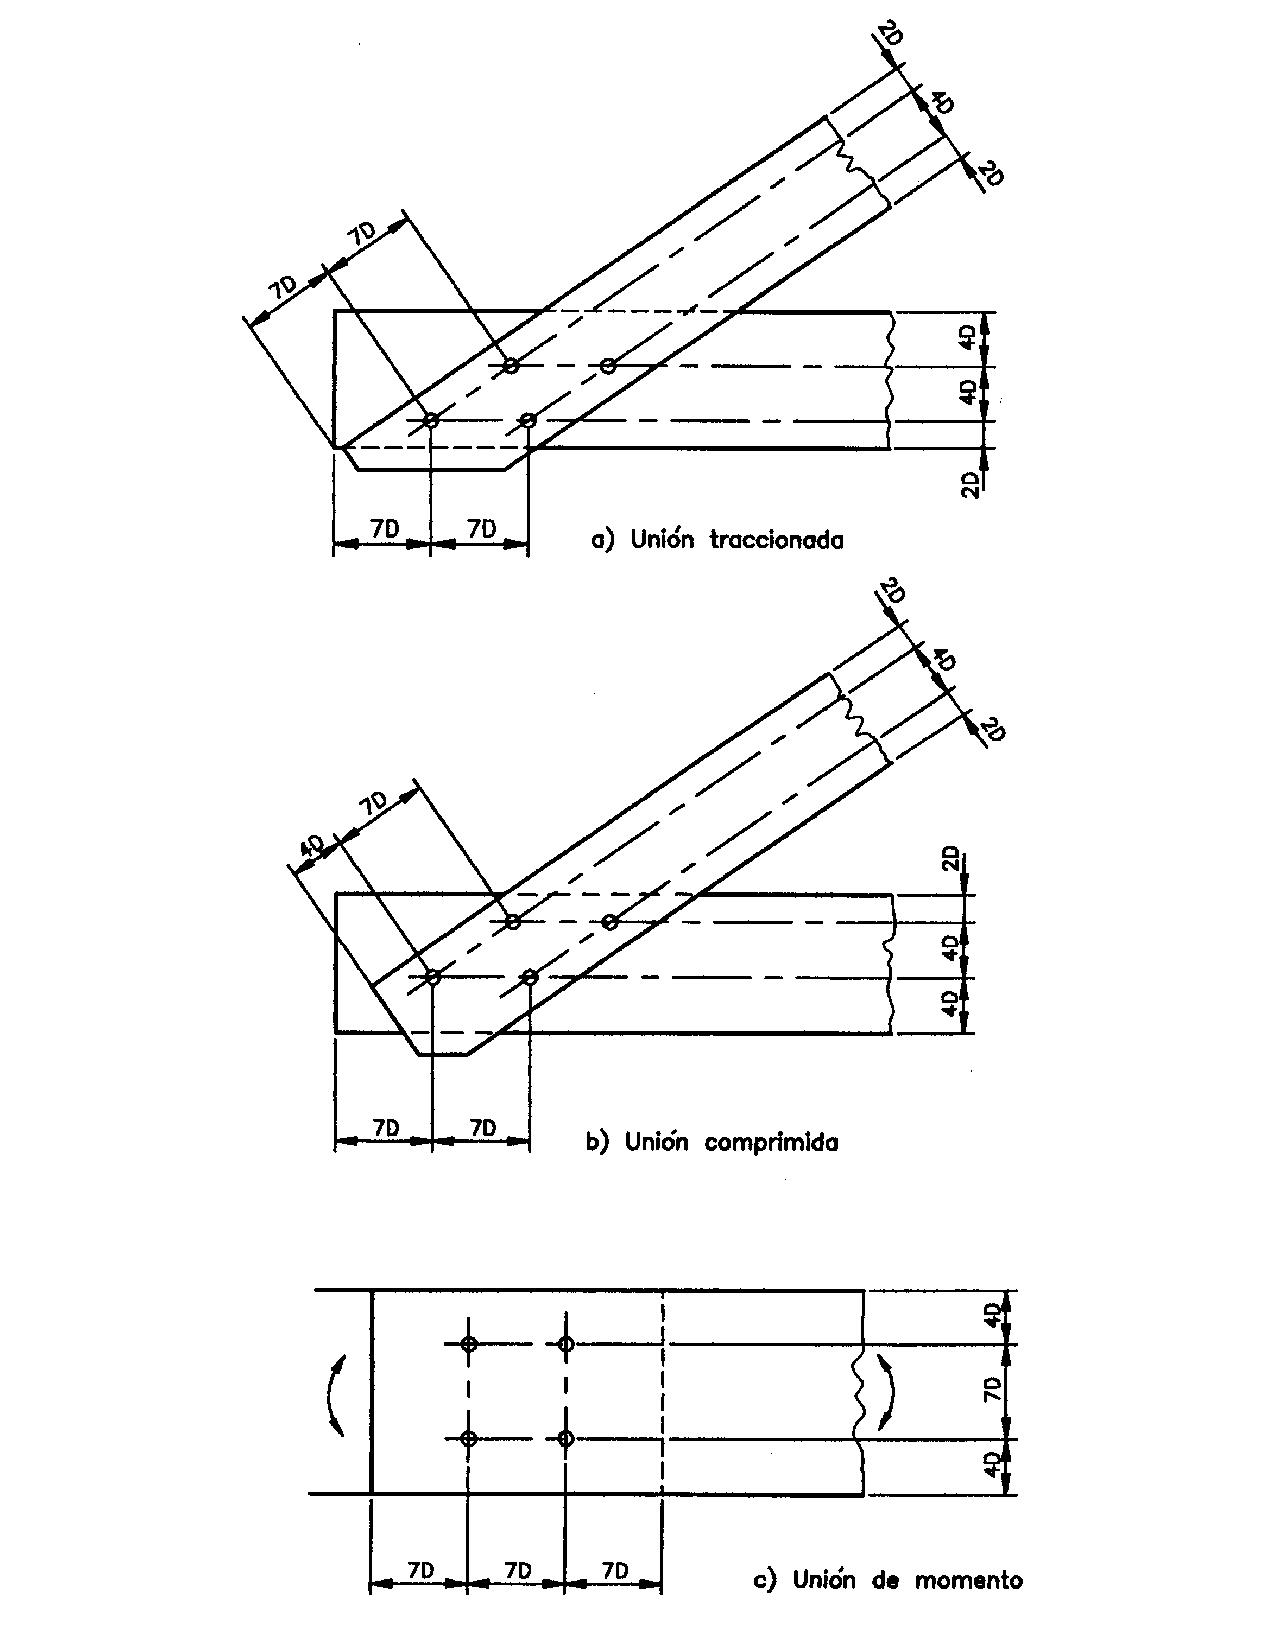
\includegraphics[width=1\linewidth, angle=1,origin=c]{Imagenes/figura_26.pdf}%
\caption{Espaciamientos mínimos ntre pernos, barras de acero, tirafondos y a los bordes. \cite{nch1198}}
\label{fig:nch_26}
\end{figure}

\subsection{Uniones con tirafondos}
\label{sec:tirafondos}
Los tirafondos son un tipo de unión mecánica similar a un tornillo, del cual se diferencia porque su longitud total está dividida en una zona roscada y otra lisa llamada vástago, como se muestra en la figura \ref{fig:nch_28}. Las especificaciones y cálculos indicado en esta norma son válidos para tirafondos que cumplan con las características del anexo M de la norma.

Para obtener los valores de diseño para este tipo de unión, es necesario clasificar las especies madereras utilizadas según su densidad anhidra $\rho_o$ (obtenidas en el anexo E), de acuerdo a la tabla 38 de la norma.

\begin{figure}[H]
\centering
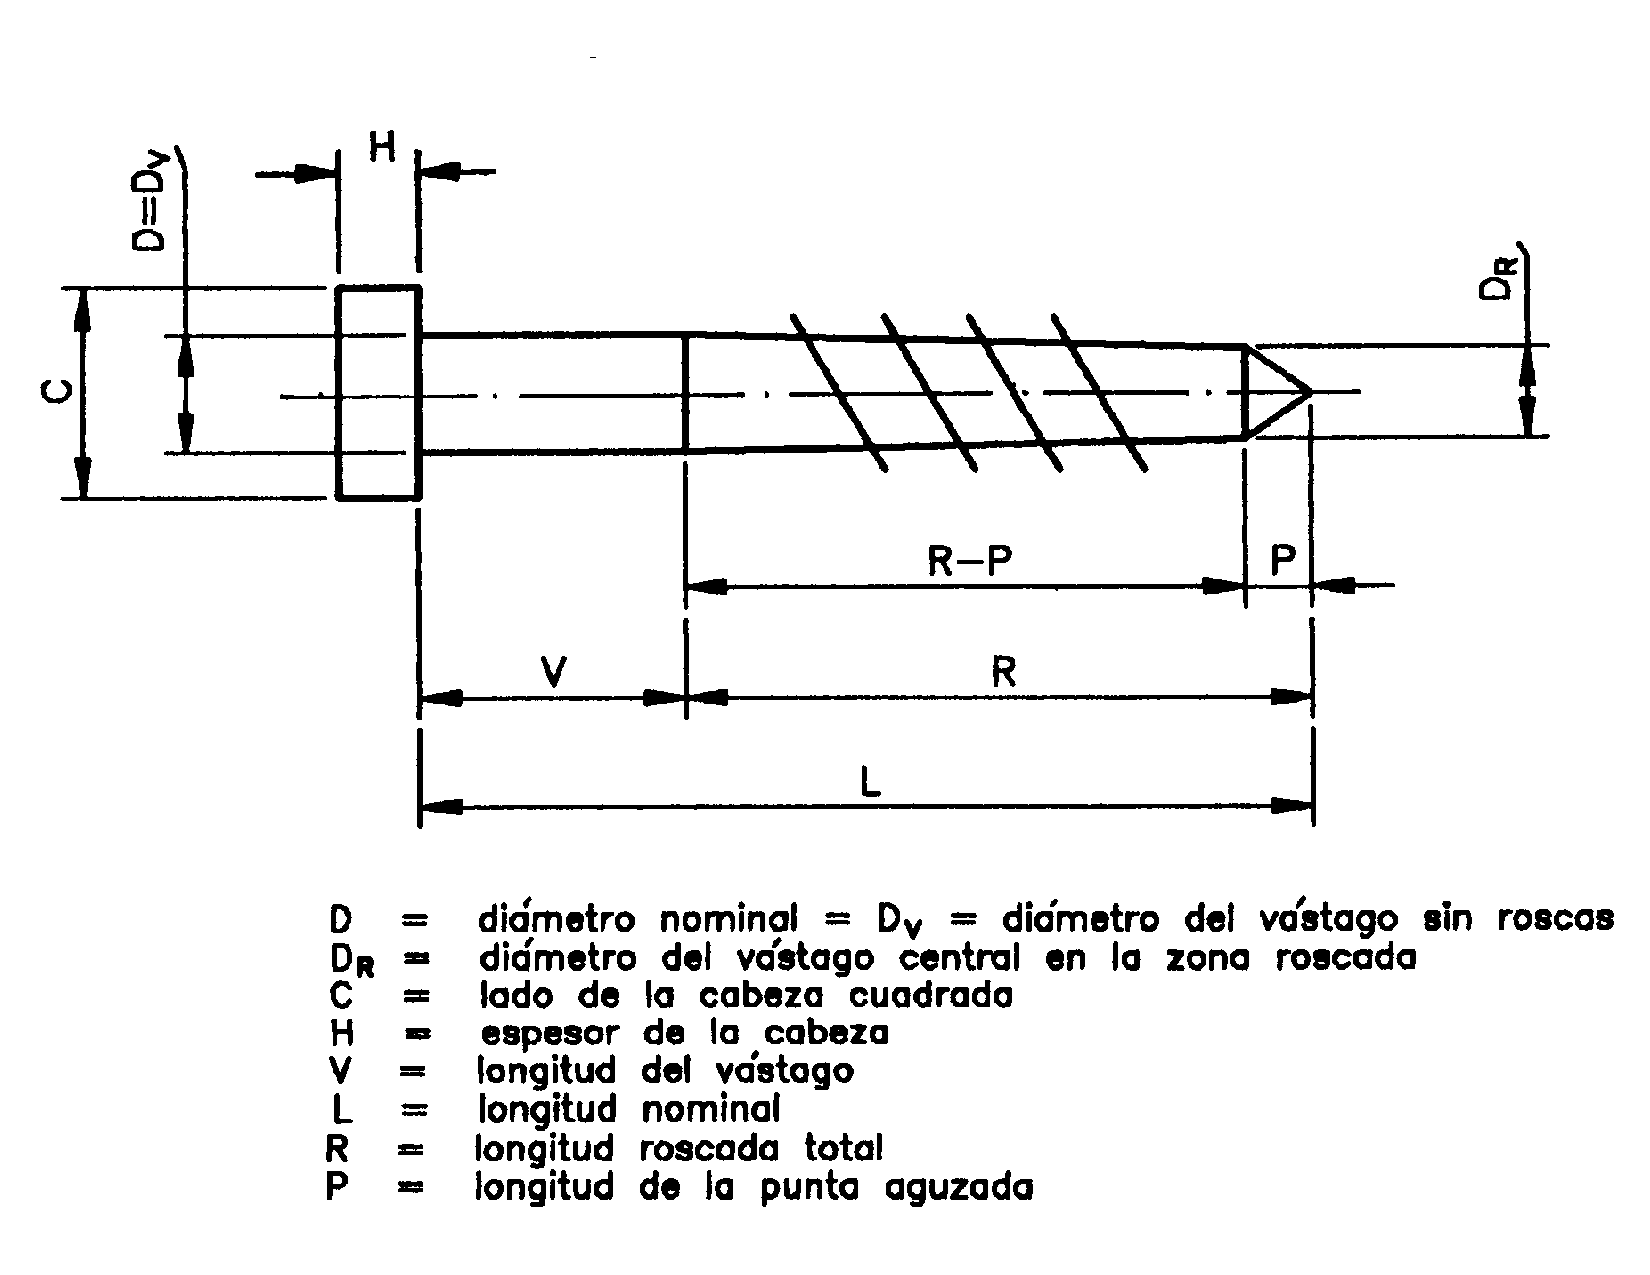
\includegraphics[width=0.9\linewidth]{Imagenes/figura_28.pdf}%
\caption{Esquema de un tirafondo. \cite{nch1198}}
\label{fig:nch_28}
\end{figure}

\subsubsection{Perforaciones guía}
Los tirafondos deben ser instalados en perforaciones guías con las características siguientes:
\begin{itemize*}
	\item El agujero en donde se alojará el vástago del tirafondo debe tener el mismo diámetro $D$ de dicho vástago y una profundidad igual a la longitud, $V$, de la zona sin rosca del tirafondo.
	\item El agujero para la zona con rosca del tirafondo debe tener una profundidad de al menos igual a la longitud de la zona roscada del tirafondo, $R-P$ y un diámetro comprendido entre:
	\begin{itemize*}
		\item 40\% - 70\% del diámetro del vástago para las especies del grupo A de la tabla 38 de la norma.
		\item 60\% - 75\% de dicho diámetro para las especies del grupo B.
		\item 65\% - 85\% para las de los grupos C y D.
	\end{itemize*}
\end{itemize*}
Para tirafondos de diámetros iguales o mayores que $3/4"$ (ver anexo M) ocupar los porcentajes del límite superior de los intervalos señalados. Cuando los tirafondos con diámetros menores o iguales a $3/8"$ colocados en maderas del grupo A y B son sometidos a extracción directa, se puede evitar la perforación guía si los espaciamientos entre tirafondos y las distancias a los bordes de la pieza cumplen con las seccionas \textbf{10.5.4.1} y \textbf{10.5.4.2}.
La zona con rosca debe ser colocada en la perforación guía con una llave de tuerca. Se prohibe la aplicación de golpes de martillo en esta operación. Para facilitar la introducción y evitar daños en el tirafondo se acepta el empleo de lubricantes en la rosca o en la perforación.

\subsubsection{Arandelas}
Las arandelas siguien las especificaciones de la tabla 34 de la norma, señaladas en la sección de la unión con pernos, excepto que se dipongan planchas de acero.

\subsubsection{Solicitaciones de extracción lateral}
La carga admisible de extracción lateral de tirafondos colocados en su eje normal a las fibras de la madera y sometidos a una carga paralela a dichas fibras, se obtiene a partir de la siguiente expresión:
\begin{equation}\label{eq:pel_ad}
	P_{el,ad}=K\cdot D^2 \cdot 10^{-3} \qquad \text{(kN)}
\end{equation}
Donde $P_{el,ad}$ es la carga admisible de extracción lateral, $D$ el diámetro del vástago del tirafondo, en mm, y $K$ es la constante que depende de la densidad anhidra y cuyo valor se puede obtener de la tabla 39 de la norma.
Las cargas admisibles son aplicables sólo si se cumplen las siguientes condiciones:
\begin{enumerate}
	\item El espesor $e_L$ de la pieza lateral atravesada por el tirafondo es igual a $3,5D$.
	\item La profundidad mínima de penetración en la pieza principal (la que recibe la punta del tirafondo), asciende a:
	\begin{itemize}
		\item $7D$ en maderas de los grupos C y D.
		\item $11D$ en maderas de los grupos A y B.
	\end{itemize}
	\item La penetración del vástago es completa en la pieza lateral, sin que él penetre en la pieza principal, como se muestra en la figura 29 de la norma. 
\end{enumerate}

En caso de no cumplirse las condiciones señaladas, es necesario multiplicas el valor $P_{el,ad}$ obtenido en la ecuación \ref{eq:pel_ad} por los factores de modificación correspondientes.
\begin{enumerate}
	\item \textbf{Factor de modificación por espesor de la pieza lateral, $K_{te}$}\\
	Para espesores de piezas laterales diferentes a $3,5D$, se debe utilizar la tabla 40 de la norma.
	\item \textbf{Factor de modificación por penetración del vástago en la pieza principal, $K_{tv}$}\\
	Cuando el vástago toca la pieza principal, se debe utilizar el factor de modificación señalado en la tabla 41 de la norma, utilizando la razón $P_v / D$ como dato de entrada, donde $P_v$ se especifica en la figura 30 de la norma.	
\end{enumerate}

Además, siempre se debe multiplicar la carga admisible a la extracción lateral de la ecuación \ref{eq:pel_ad} por el factor de modificación por diámetro, $K_{tD}$, que se entrega en la tabla 42 de la norma.

Cuando $P_{el,ad}$ es calculado para tirafondos colocados con su eje paralelo a las fibras de la madera de la pieza principal y sometidos a una carga normal a dichas fibras se debe considerar igual a $2/3$ de la multiplicación de $P_{el,ad} \cdot K_{tD}$. Por otro lado, cuando se usen cubrejuntas metálicas, la carga admisible de extracción lateral se debe amplificar en un 25\% para cargas paralelas de la dirección de la fibra. Esta mayoración no se aplica sobre la carga admisible normal a la dirección de la fibra.

\subsubsection{Solicitaciones de extracción directa}
La carga admisible de extracción directa de tirafondos colocados con su eje normal a las fibras de la madera, se determina con la expresión:
\begin{equation}\label{eq:ped_ad}
	P_{ed,ad} = \frac{\rho_{o}^{1,5} \cdot D^{0,75} \cdot l_{crit}}{978} \cdot 10^{-3} \qquad \text{(kN)}
\end{equation}
Donde:

\begin{align*}
&P_{ed,ad} &= \quad &\text{carga admisible de extracción directa}\\
&\rho_o &= \quad &\text{Densidad anhidra de la madera en} kg/m^3 \\
&D &= \quad &\text{Diámetro del vástago del tirafondo en mm}\\
&l &= \quad &\text{Longitud de penetración de la zona roscada del tirafondo (R-P) en la madera, en mm}\\
&l_{crit} &= \quad &\text{Longitud de penetración de la zona roscada que desarrolla la capacidad admisible de}\\
& & & \text{tracción  en la sección transversal crítica del tirafondo, según tabla 43 de la norma.}
\end{align*}

En caso que la solicitación de la extracción directa quede con su eje colocado paralelo a las fibras de la madera, se debe considerar una carga admisible igual al 75\% de aquella calculada para tirafondos colocados con su eje normal a las fibras de la madera.

\subsubsection{Combinación de solicitaciones de extracción directa y lateral}
Cuando un tirafondo esté solicitado tanto en extracción directa como lateral, el análisis se realiza por separado, no debiendo exceder la carga de diseño de extracción para ninguno de los dos casos.

\subsubsection{Espaciamiento}
Las distancias entre tirafondos y entre tirafondos y bordes debe seguir lo establecido en la tabla 36 del capítulo de pernos de la norma, donde se reemplaza el diámetro del perno por el diámetro del vástago.
